% !TeX encoding = ISO-8859-1
\chapter{Einleitung}
\label{chap:einleitung}

\section{Ausgangssituation}

In dieser Projektarbeit soll zuerst ein Vergleich der Eigenschaften �hnlicher
Betriebssysteme wie FreeRTOS, RIOT, Kontiki, usw. vor allem bez�glich der Unterst�tzung der
verschiedenen Netzwerkprotokolle gemacht werden. Anschliessend sind geeignete Boards f�r das Betriebssystem Zephyr zu evaluieren.
Zu Demonstrationszwecken soll am Schluss mit dem ausgew�hlten Board eine Demo-App entwickelt werden.


\vspace{20mm}
\begin{figure}[h]
	\centering
	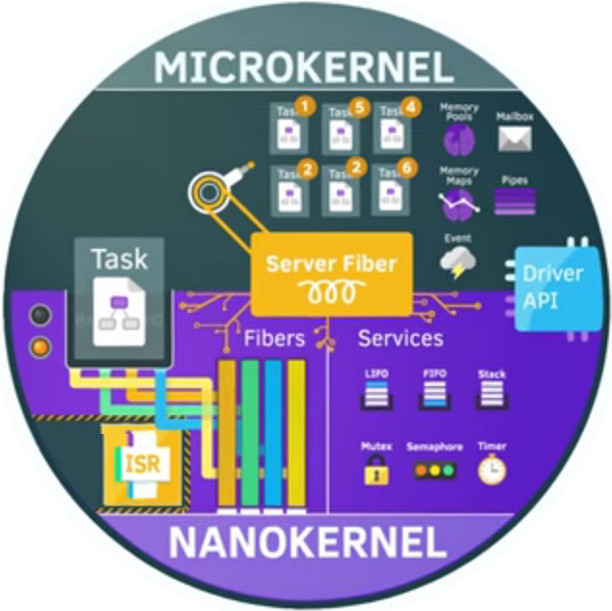
\includegraphics[width=0.7\linewidth]{bilder/zephyr_rtos_concept.jpg}
	\caption{�bersicht �ber den Nano- und Microkernel des Zephyr-Betriebssytems}
	\label{fig:components}
\end{figure}
\vspace{5mm}

\section{Projektbegr�ndung}

F�r das Modul ''Projektarbeit und System Engineering BTE5511'' wird ein Projekt bearbeitet. Das Projekt wurde w�hrend der unterrichtfreien Zeit ausgeschrieben und den jeweiligen Studierenden zugewiesen. Das Ziel dieser Arbeit ist die Studierenden mit Projektarbeiten vertraut zu machen.

Im Rahmen der Projektarbeit des 5. Semesters realisiert dieses Projekt einen Vergleich zwischen dem Zephyr-Betriebssystem und �hnlichen Betriebssysteme wie FreeRTOS, RIOT, Kontiki, usw. Ausserdem sollen die F�higkeiten des Zephyr-ROTS in bestehender Form ausgetestet werden. Spezielle Beachtung soll den f�r das Internet der Dinge wichtigen Kommunikationsprotokollen wie BLE und Near Field Communication (NFC) getestet werden. Anschliessend sind geeignete Boards f�r das Betriebssystem Zephyr zu evaluieren. Des Weiteren sollen die zwei unterschiedlichen Kernel des Zephyr-Betriebssystems verglichen werden. Zu Demonstrationszwecken soll am Schluss mit dem ausgew�hlten Board eine kleine Demo-App entwickelt werden.


\section{Kundenanforderungen}

Mit diesem Projekt soll intern das Know-how f�r das Zephyr-Open-Source-Betriebssystem, welches ein solides OS f�r IoT Ger�te mit geringen Ressourcen bereitstellt und eine echtzeitf�hige Kombination aus Nano- und Microkernel nutzt, ausgebaut werden. Das gesammelte Wissen wird dem Fachbereich Elektrotechnik f�r den Unterricht zur Verf�gung gestellt. Eine weitere Kundenanforderung ist es, dass wir bei unserer Projektarbeit nur Open-Source Software und Softwaretools verwenden, somit m�chten wir unser Wissen auch der Open-Source-Community zur Verf�gung stellen.

\vspace{5mm}

Die Ziele sind:

\begin{itemize}
	\item Einarbeitung in das Betriebssystem Zephyr.
	\item Erstellen einer Vergleichstabelle mit den wichtigsten Eigenschaften der verschiedenen
	RTOS.
	\item Evaluation geeigneter Boards f�r das Zephyr Betriebssystem f�r eine IoT.
	\item Entwicklung einer Demonstrationsapplikation, basierend auf dem ausgew�hlten Board.
\end{itemize}